\section{\name Prototype Implementation}
\label{sec:prototype}


\begin{figure}[t]
    \begin{center}
        \begin{subfigure}{0.4\textwidth}
        \centering
            %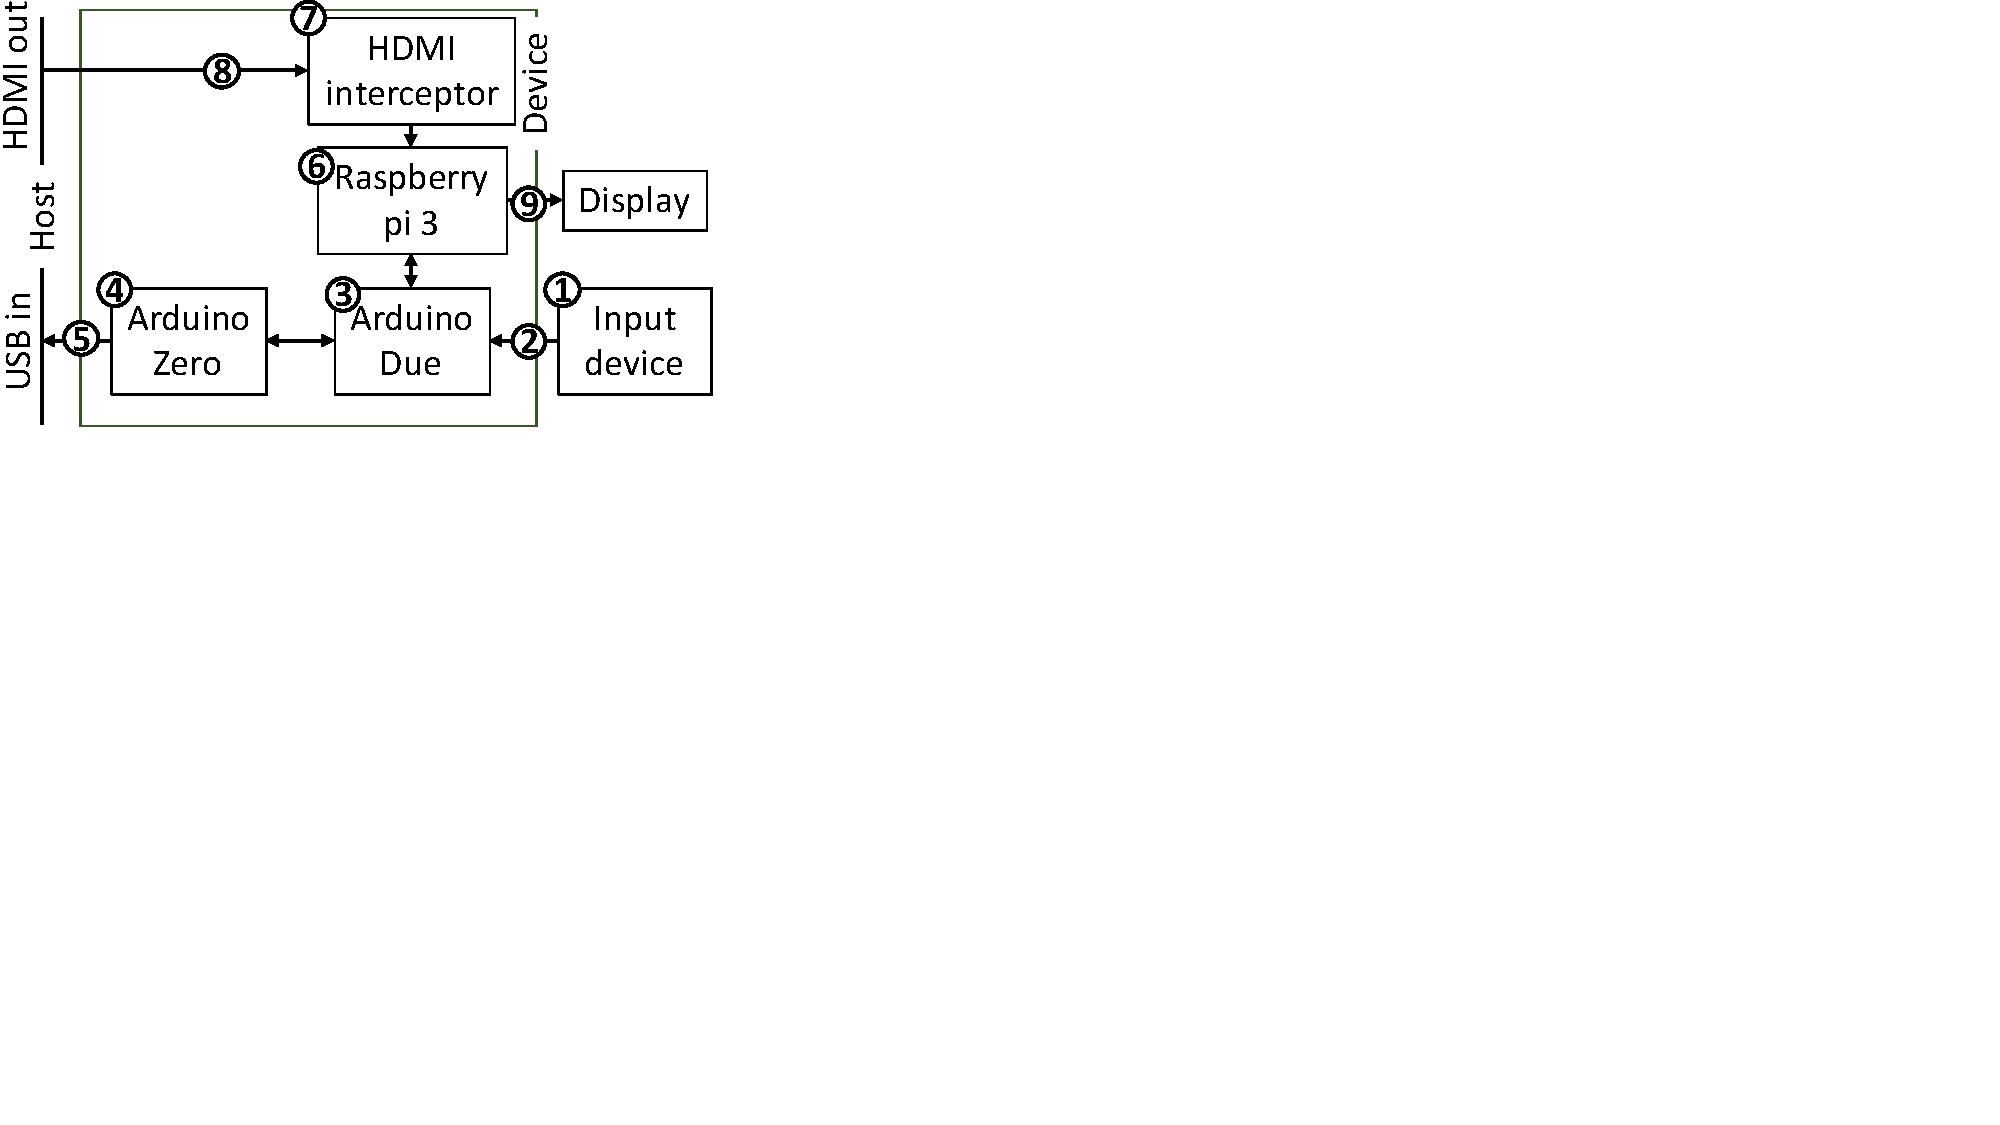
\includegraphics[trim={0 12cm 21.7cm 0}, clip, scale=0.45]{setUpBlock.pdf}
            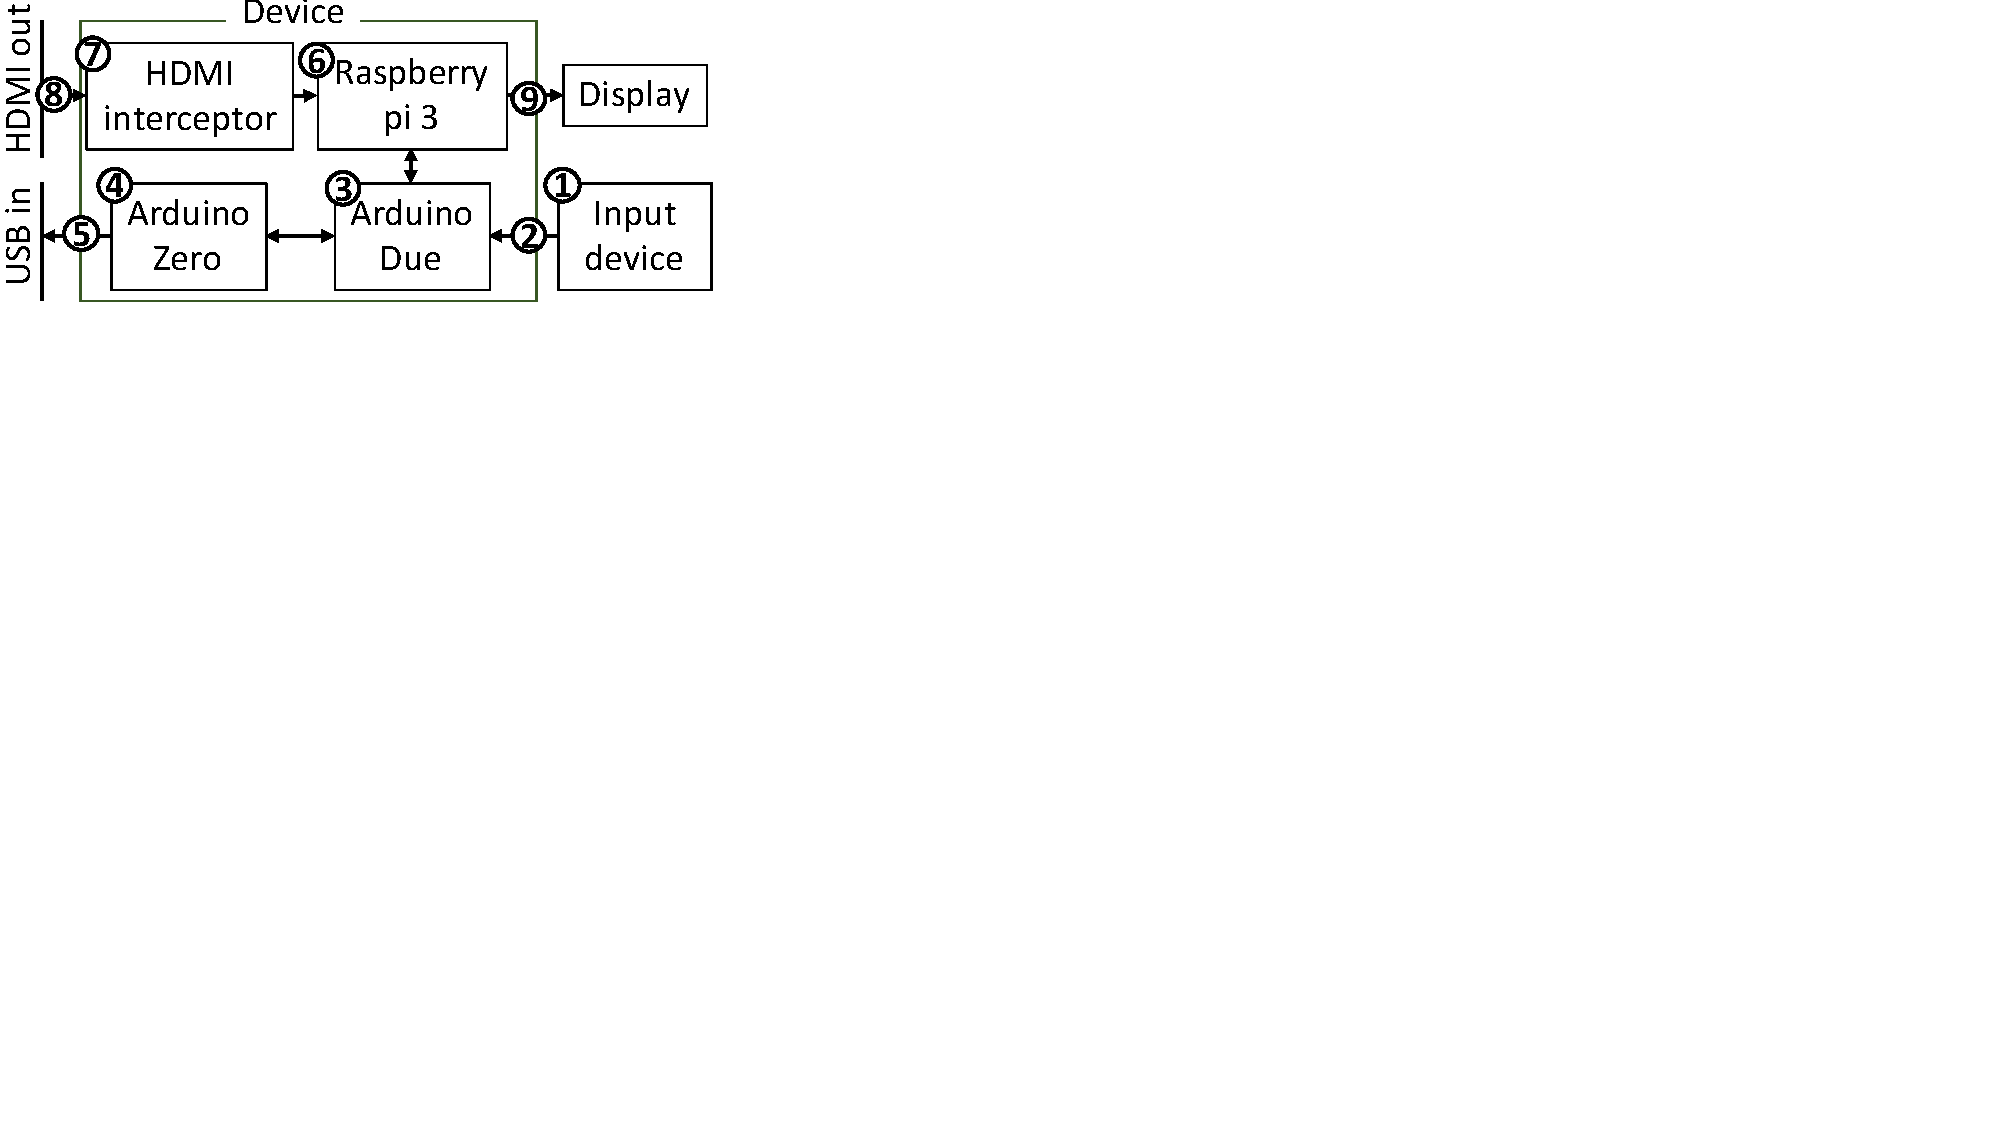
\includegraphics[trim={0 13.7cm 21.7cm 0}, clip, scale=0.45]{setUpBlock_1.pdf}
            \caption{The figure shows the basic components and connections between them in our \name prototype.}
            \label{fig:prototypeArch}    
        \end{subfigure}
    \end{center}
    
    %\vspace{1em} 
    
    \begin{center}
        \begin{subfigure}{0.4\textwidth}
        \centering
        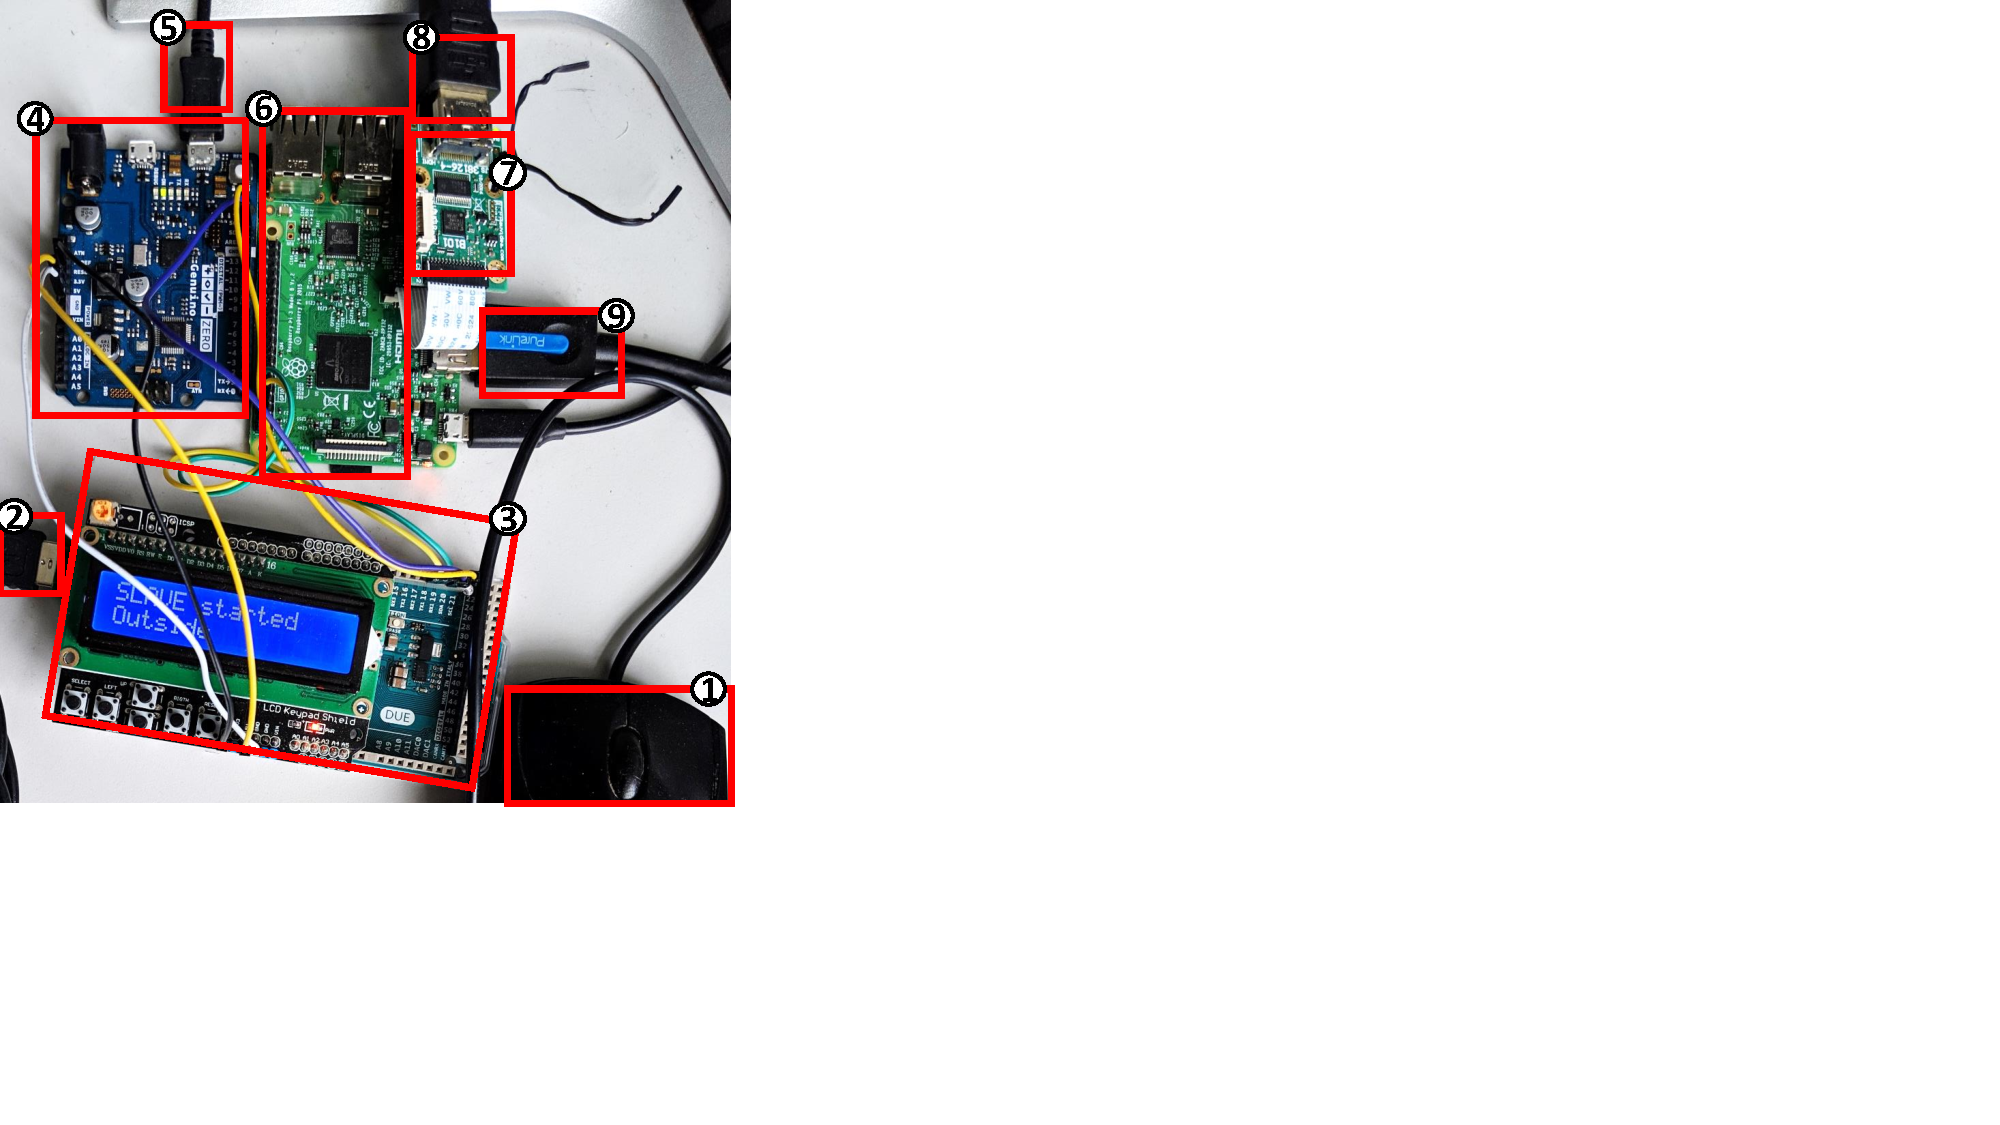
\includegraphics[trim={0 6.6cm 21.5cm 0}, clip, scale=0.55]{setUp_1.pdf}
        \caption{The figure shows \name prototype that employs Arduino Due and Zero microcontroller board and a Raspberry Pi 4 SBC. The highlighted numbers correspond to the labels in Figure~\ref{fig:prototypeArch}.}
        \label{fig:prototype}
    \end{subfigure}
    \end{center}
    \vspace{-1em}
    
    \caption{\textbf{\name prototype}. Figure~\ref{fig:prototypeArch} and~\ref{fig:prototype} shows the component diagram and a photo of the actual \name prototype respectively.} 
    \label{fig:prototypeAll}
    \spacesave
\end{figure}

\myparagraph{Setup} Here, we describe our prototype implementation of \name as an auxiliary device. Figure~\ref{fig:prototypeAll} depicts the \name prototype in two parts: Figure~\ref{fig:prototypeArch} shows the block diagram of our prototype with various components and connections, and Figure~\ref{fig:prototype} shows a photo of the actual prototype that highlights all the components described in the block diagram. The prototype \device is connected to a desktop computer with 3.40 GHz Intel Core i7-6700 processor with 8 GB RAM running Ubuntu 18.04.2 LTS. The \device uses off-the-shelf devices and has the following components (we use the same numbering as shown in Figure~\ref{fig:prototypeArch} and  Figure~\ref{fig:prototype}):

\begin{mylist}
 
  \item \textbf{Computing component.} We use a Raspberry Pi 4 (\six) to implement the computing component that executes all the \device logic that includes analyzing the HDMI frames, rendering the overlays, executing the \tls protocol, etc. One could use an ASIC to further improve the performance and reduce the code base of the component. The Pi is connected to the display over HDMI (\nine) interface. The code base of the Pi primarily consists of Python and Java.
  
  \item \textbf{Input interceptor.} The input interceptor is composed of an Arduino Due (\three) and an Arduino Zero (\four) that is connected to the input device over \usb (\two) interface. The input interceptor has a \usb out interface that connects to the host (\five) that relays all the user inputs to the host. 

  \item \textbf{HDMI interceptor.} The HDMI interceptor (\seven) is implemented using a B101 HDMI to CSI-2 Bridge~\cite{b101} that takes the HDMI channel (\eight) from the host and convert it to the camera input signal to the Raspberry Pi 4.  
 
\end{mylist}

\subsection{Implementation of \name Components}
\label{sec:prototype:impl}


In the following, we provide the implementation details of the \name components presented in the previous sections. Detailed implementation is provided in Appendix~\ref{appendix:implementation}.

\subsubsection{\bfseries QR code generation \& UI specification}
\label{sec:prototype:impl:qr}

QR code generation phase is executed by \name JS that transforms the UI elements of a sensitive web form to a UI specification encoded in a QR code (we use QRCode.js, a \js library to produce QR codes). Section~\ref{sec:systemDesign:transformation} provides the high-level concept of generating the QR code from the webpage UI elements. UI elements that require IO integrity protection can be marked by the developers in the \html source. As illustrated in Figure~\ref{fig:transformation}, the \html UI elements: `\texttt{Sensitive field 1}' and `\texttt{Sensitive field 2}' have the additional attribute \texttt{protect=``true''}. %(one concrete example is illustrated in Figure~\ref{fig:transformation}). 

The \name JS iterates through the HTML elements that have the \texttt{protect} attribute enabled and extracts the information such as the name of the label or the type of the UI element. \device uses preloaded size parameters to specify the size of a text field, button, etc. in case the size is not explicitly mentioned in the HTML source. One important attribute for a UI element in the specification is the \texttt{trigger}. For example, in Specification~\ref{snippet:UISpecification}, the \texttt{OK} and the \texttt{cancel} buttons have an attribute \texttt{trigger}. This attribute is Boolean can be either \texttt{true} (corresponding to \texttt{OK}) or \texttt{false} (corresponding to \texttt{Cancel}) value. The value \texttt{true} denotes that the \texttt{OK} button can submit the values that are provided by the user. The \texttt{false} attribute denotes that hitting the \texttt{cancel} button abort the form altogether. 

The QR code generation phase is between \one and \two in Figure~\ref{fig:transformation} where the \name JavaScript snippet transforms the UI elements to a UI specification language in a QR code that can be interpreted by the \device. The UI specification corresponding to the \html source (in Figure~\ref{fig:transformation}) is provided in Specification~\ref{snippet:UISpecification}. Note that the specification is highly flexible, allowing adjustable size for the form, individual UI elements, gaps between them, etc. This allows the \device to faithfully recreate the UI that is very close to the actual form UI that the served by the web severer. 
%Such allows negligible user habituation. 

\subsubsection{\bfseries Bitmap generation}
\label{sec:prototype:impl:bitmap}

The \device reads the QR code from the HDMI frame and generate the UI overlay bitmap from it. We have used the \texttt{piCamera} library to intercept the HDMI frames and generate the UI on top of it. Our \name prototype implements the most frequently used HTML input elements~\cite{html_elements} that are common in sensitive forms. 

\subsubsection{\bfseries Detection of mouse pointer}
\label{sec:prototype:impl:mouse}

Initially, when the system boots up the \device perform the calibration phase (see Section \ref{sec:systemDesign:analysis:calibration}) to synchronize its coordinates of the pointer with the host. The detection of the mouse pointer is implanted partially on the raspberry pi 4 (\six in Figure~\ref{fig:prototypeAll}), while the mouse intercepting is done in the Arduino Due (\three in Figure~\ref{fig:prototypeAll}). The Due gathers the raw mouse data (in terms of displacement measurements $(\Delta x_i, \Delta y_i)$) and sends them to the Pi over \texttt{Serial} interface.  To guarantee that the \device and the host interpret displacement events likewise, the Pi performs an adjustment operation. This operation consists of the \device detecting the exact position of the host pointer in the HDMI frame by analyzing a small square of the frame (50 x 50px) around its pointer coordinates. Considering that the \device gets raw HDMI frames and pointer images are static, we use the lightweight \texttt{template matching} algorithm of the OpenCV library for the detection.

\subsubsection{\bfseries Implementation of the upstream channel}
\label{sec:prototype:impl:upstream}

 The \emph{upstream} channel, i.e., the data from the \device to the remote server is transmitted using the \name JavaScript snippet that is served by the remote web server. The \name JavaScript snippet uses a hidden text field to accept data coming from the \device. The \device emulates itself as a composite human interface device (HID) when it is connected to the host. The \device emulates keystrokes that transmit encoded data (base64) to the \name JavaScript snippet that is sent to the remote server via \texttt{XMLHttpRequest} call.

\begin{figure}[t]
\centering
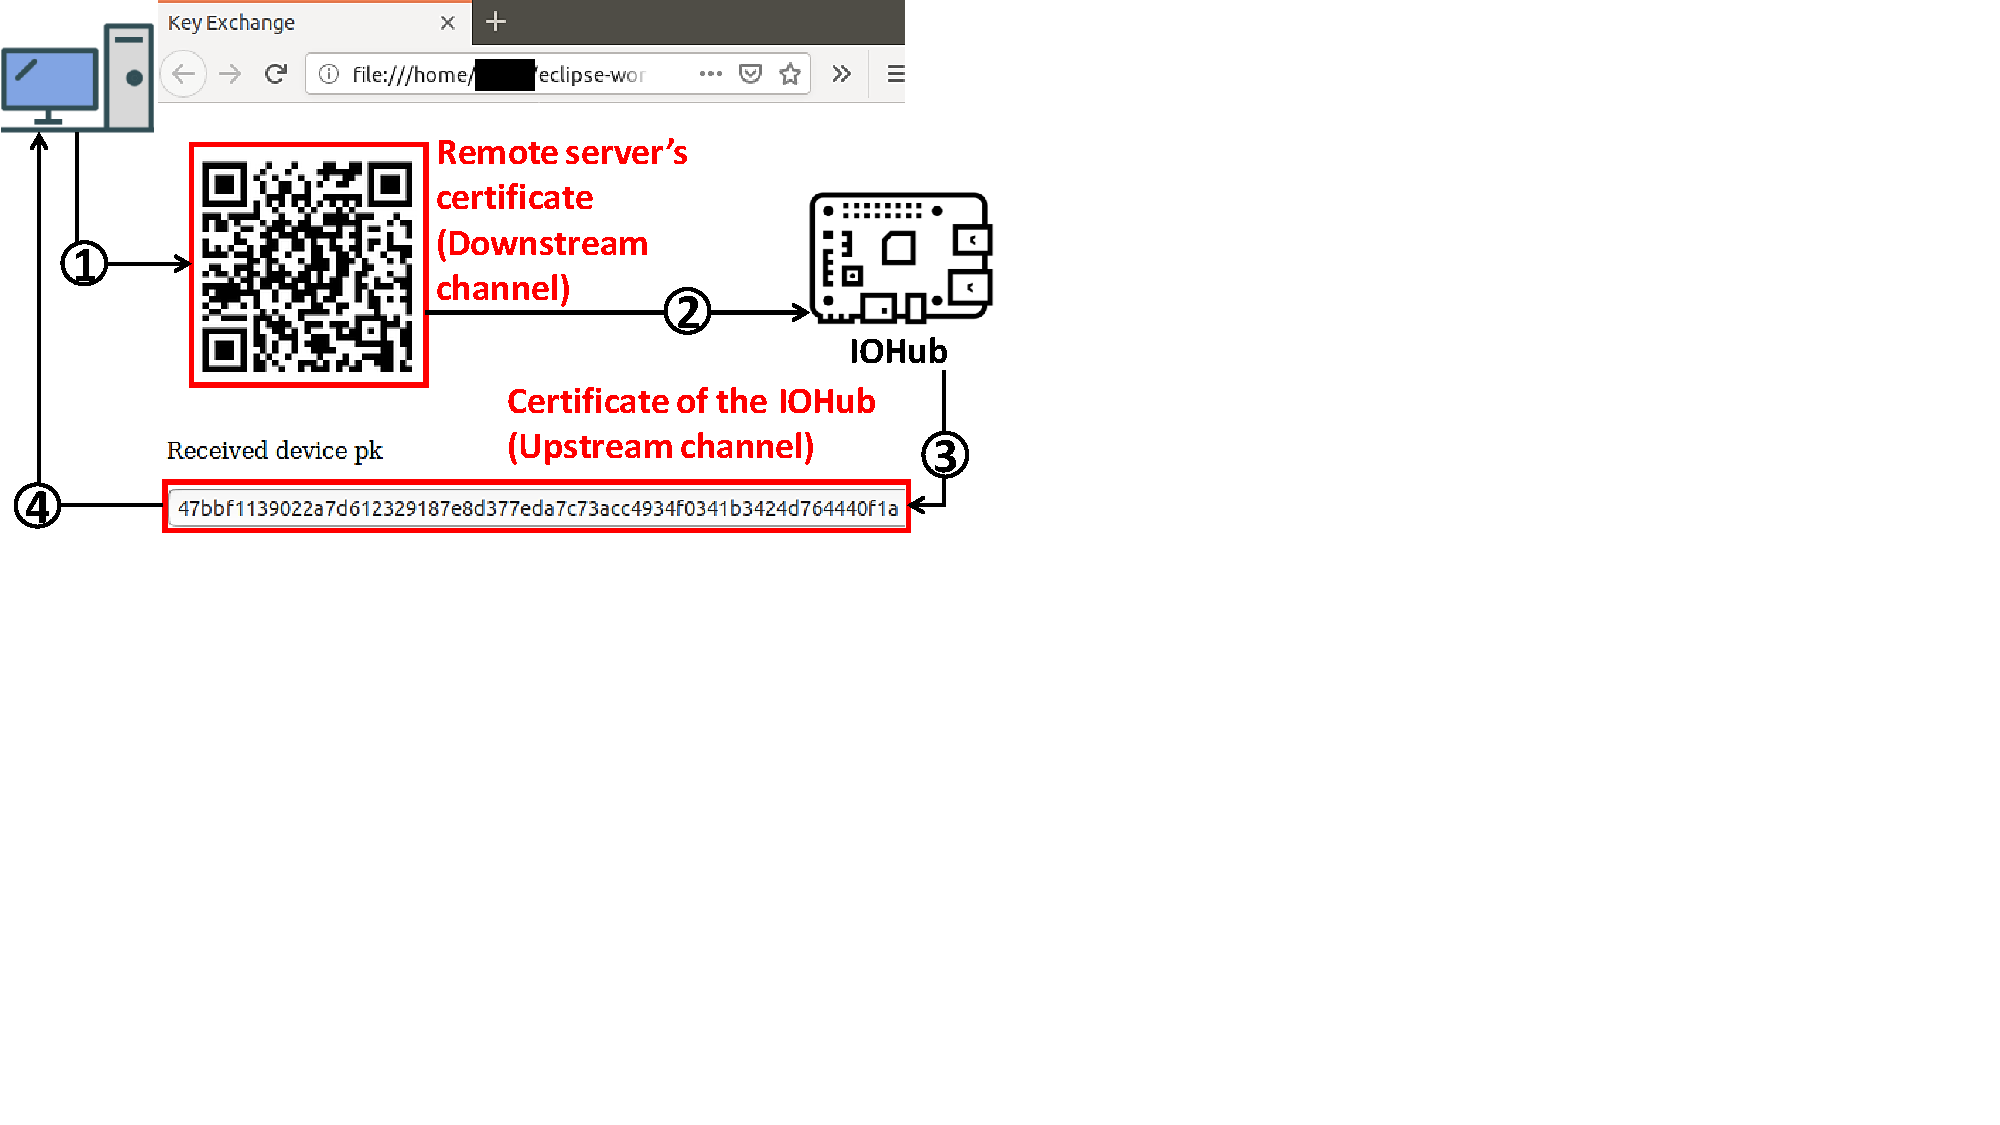
\includegraphics[trim={0 10cm 17cm 0}, clip, width=0.85\linewidth]{keyExchange_1.pdf}
\caption{\textbf{Establishing \tls.} A snapshot of the key exchange web page that is used to communicate the public certificates of the device and the remote server.}
\spacesave
\label{fig:keyExchange}
\centering
\end{figure} 

\subsubsection{\bfseries Establishing \tls}
\label{sec:prototype:impl:tls}

For the IO confidentiality, the \device and server create a \tls channel. When the user opens up a secure webpage, key exchange is the first step that takes place. We assume that the remote server already has the \device's certificate, or some offline registration takes place. An instance of the key exchange protocol of \name is illustrated in Figure~\ref{fig:keyExchange}. The flow of the key exchange mechanism is as the following:
\vspace{-10pt}
\begin{mylist}
  \item[\one] The server delivers a web page with a QR code that encodes the signed public key of the server (server hello in TLS). 
  \item[\two] The device captures every frame until it detects a QR code. Then, it decodes the QR code and verifies the public key and derives the shared secret using Diffie-Hellman protocol~\cite{blake1998authenticated}. 
  \item[\three] The device then sends its signed public certificate to the host, which forwards it to the server.
  \item[\four] The remote server gets the signed certificate from the \device, verifies it, and finally derives the shared secret.
\end{mylist}
